\documentclass{article}
\usepackage{tikz, comment}
\usepackage{pifont}
\usepackage{fontspec}
\usetikzlibrary{arrows, decorations.markings, decorations.pathreplacing}
\begin{comment}
:Title: Not defined yet
:Tags: symmetry;side;isosceles;figure;curve;closed;between
:Author: Prof.Hu Ji-shan, HKUST
:Slug: No name yet

Description Here.........
\end{comment}
\begin{document}\centering

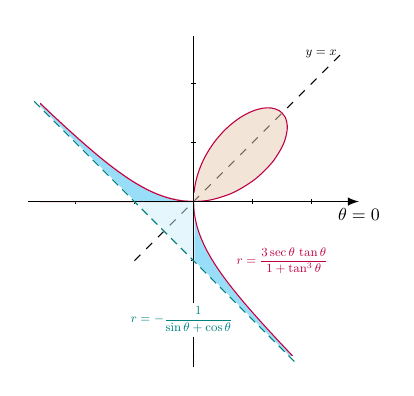
\begin{tikzpicture}[>=latex,xscale=.5*1.5, yscale=.5*1.5][font=\sf\small]

%\draw[xstep=1cm,ystep=1cm,color=gray!80] (0, -1) grid (8, 8);


%\draw[purple, samples=100, smooth, domain=-0.5:0, variable=\t]
% plot ({2*(\t)/(1+(\t)^3)}, {2*(\t)^2/(1+(\t)^3)})--(0,0);

\draw[->] (-2.8, 0) -- (2.8, 0)node[below, scale=0.7] {$\theta=0$} ;
\draw[] (0, -2.8) -- (0, 2.8)node[left] {} ;

\foreach \x in {-2,-1,1,2}
\draw (\x,2pt/1.5) -- (\x,-2pt/1.5)
node[anchor=north] {}%{\tiny$\x$}
;

\foreach \x in {}
\draw (\x,2pt*2) -- (\x,-2pt*2)
node[anchor=south] {\tiny$\x$}
;
\foreach \y in {-2,-1,1,2}
\draw (-2pt/1.5,\y) -- (2pt/1.5,\y)
node[anchor=east] {}%{\tiny $\y$}
;

\clip[] (-2.7, -2.7) rectangle (2.7, 2.7);

\draw[densely dashed, teal, samples=100, smooth, domain=-2.7:2.7, variable=\x]
plot ({\x}, {-\x-1});

\draw[dashed, samples=100, smooth, domain=-1:2.5, variable=\x]
plot ({\x}, {\x}) node[left, scale=0.5] {$y=x$};
\node[teal, scale=0.5] at (0.75, -2.5) {$y=-x-1$};

\clip[] (-2.6, -2.6) rectangle (2.6, 2.6);

\draw[white, fill=brown!40, fill opacity=0.5, samples=150, smooth, domain=0:20, variable=\t]
plot ({3*(\t)/(1+(\t)^3)}, {3*(\t)^2/(1+(\t)^3)})--(0,0);

\draw[purple, samples=150, smooth, domain=-0.9:20, variable=\t]
plot ({3*(\t)/(1+(\t)^3)}, {3*(\t)^2/(1+(\t)^3)});

\draw[white, fill=cyan!40, samples=150, smooth, domain=-0.9:0, variable=\t]
plot ({3*(\t)/(1+(\t)^3)}, {3*(\t)^2/(1+(\t)^3)})--(-2.6, 0);

\draw[purple, samples=150, smooth, domain=-0.9:0, variable=\t]
plot ({3*(\t)/(1+(\t)^3)}, {3*(\t)^2/(1+(\t)^3)})--(-2.6, 0);

\draw[white, fill=white, samples=100, smooth, domain=-2.7:-1, variable=\x]
plot ({\x}, {-\x-1})--(-2.6, 0);

\draw[white, densely dashed, samples=100, smooth, domain=-2.7:-1, variable=\x]
plot ({\x}, {-\x-1});

%%%%%%
\draw[white, fill=cyan!40, samples=150, smooth, domain=-1.1:-20, variable=\t]
plot ({3*(\t)/(1+(\t)^3)}, {3*(\t)^2/(1+(\t)^3)})--(0,-2.6);

\draw[purple, samples=150, smooth, domain=-1.1:-20, variable=\t]
plot ({3*(\t)/(1+(\t)^3)}, {3*(\t)^2/(1+(\t)^3)})--(0,0);

\draw[white, densely dashed, fill=white, samples=100, smooth, domain=0:2.7, variable=\x]
plot ({\x}, {-\x-1})--(0,-2.6);

\draw [white, fill=cyan!20, fill opacity=0.5] (0,0)--(-1, 0)--(0,-1)--cycle;

\draw[->] (-2.8, 0) -- (2.8, 0);
\draw[->] (0, -2.8) -- (0, 2.8);

\draw[teal, densely dashed, samples=100, smooth, domain=-2.7:2.7, variable=\x]
plot ({\x}, {-\x-1});

\node[teal, fill=white, scale=0.5] at (-0.2, -2) {$\displaystyle r = - \frac{1}{\sin \theta + \cos \theta}$};

\node[purple, fill=white, scale=0.5] at (1.5, -1) {$\displaystyle r = \frac{3 \sec \theta \, \tan \theta}{1+\tan^3 \theta}$};

%\node[fill=white] at (-0.2/1.2, -0.2/1.2) {\tiny$0$};

\end{tikzpicture}
\end{document}